\section{Pre-compliance results}

The final radiated-emission result is shown in Figure~\ref{fig:final-radiated-plot}.
The plot includes the peak trace, the average trace, the quasi-peak limit, and the
selected final quasi-peak points. The strongest final quasi-peak point was measured at
\(480\,MHz\), where the result exceeded the practical reference limit, meaning that the
AGV failed the applied EN~61000-6-3 radiated-emission comparison in this
pre-compliance measurement. The selected final results for quasi-peak measurement are
summarised in Table~\ref{tab:emi-final-results}.

\begin{figure}[H]
\centering
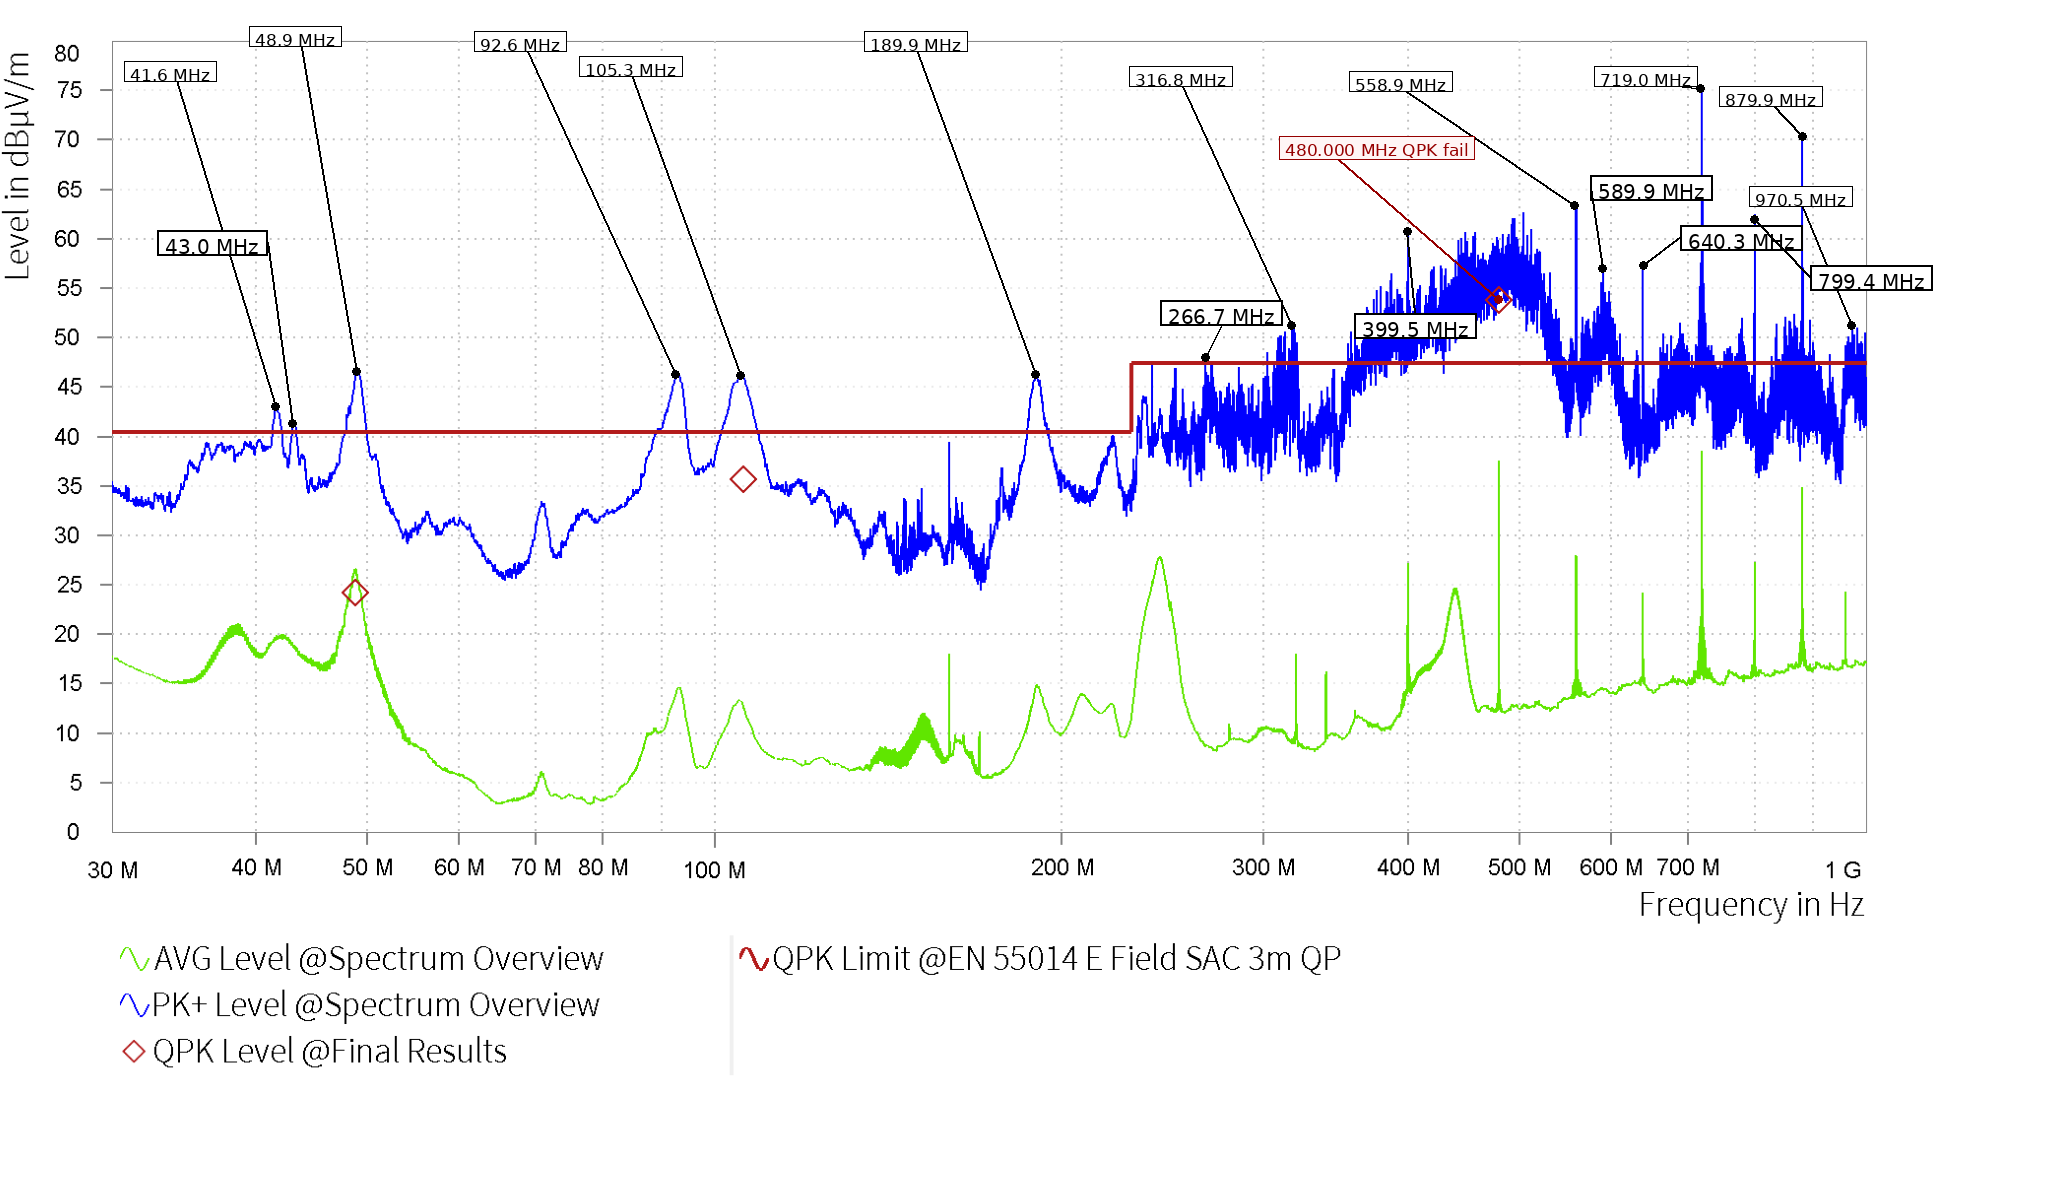
\includegraphics[width=\linewidth]{figures/final_radiated_emission_plot.png}
\caption{Radiated-emission overview plot exported from the chamber software.}
\label{fig:final-radiated-plot}
\end{figure}

\begin{table}[H]
\centering
\caption{EMI final results.}
\label{tab:emi-final-results}
\renewcommand{\arraystretch}{1.25}
\setlength{\tabcolsep}{4pt}
\resizebox{\textwidth}{!}{%
\begin{tabular}{|c|c|c|c|c|c|c|c|c|c|c|c|}
\hline
\colorbox{orange!25}{\strut Rg} &
\colorbox{orange!25}{\strut \shortstack{Frequency\\{[MHz]}}} &
\colorbox{orange!25}{\strut \shortstack{QPK Level\\{[dB$\mu$V/m]}}} &
\colorbox{orange!25}{\strut \shortstack{QPK Limit\\{[dB$\mu$V/m]}}} &
\colorbox{orange!25}{\strut \shortstack{QPK Margin\\{[dB]}}} &
\colorbox{orange!25}{\strut \shortstack{Correction\\{[dB]}}} &
\colorbox{orange!25}{\strut Polarization} &
\colorbox{orange!25}{\strut \shortstack{Azimuth\\{[deg]}}} &
\colorbox{orange!25}{\strut \shortstack{Antenna Height\\{[m]}}} &
\colorbox{orange!25}{\strut \shortstack{Meas.\ BW\\{[kHz]}}} &
\colorbox{orange!25}{\strut \shortstack{Meas.\ Time\\{[s]}}} &
\colorbox{orange!25}{\strut \shortstack{Time of\\Meas.}} \\
\hline
1 & 48.810 & 24.24 & 40.46 & \textcolor{green!50!black}{16.22} & 13.26 & V & 276.7 & 2.06 & 120.000 & 15.000 & 16:39:53 \\
\hline
1 & 105.900 & 35.71 & 40.46 & \textcolor{green!50!black}{4.75} & 11.66 & H & 91 & 2.87 & 120.000 & 15.000 & 16:25:32 \\
\hline
1 & 480.000 & 53.85 & 47.46 & \textcolor{red}{-6.39} & 18.90 & V & 217.8 & 1.00 & 120.000 & 15.000 & 16:33:06 \\
\hline
\end{tabular}%
}
\end{table}
